% Created 2026-04-24 Fri 03:00
% Intended LaTeX compiler: pdflatex
\documentclass{article}
\usepackage[utf8]{inputenc}
\usepackage[T1]{fontenc}
\usepackage{graphicx}
\usepackage{longtable}
\usepackage{wrapfig}
\usepackage{rotating}
\usepackage[normalem]{ulem}
\usepackage{amsmath}
\usepackage{amssymb}
\usepackage{capt-of}
\usepackage{hyperref}

\usepackage{fancyhdr}
\usepackage[top=25mm, left=25mm, right=25mm]{geometry}
\usepackage{longtable}
\fancyhead[R]{}
\setlength\headheight{43.0pt}
\usepackage{tabularx}
\usepackage{longtable}
\author{Jami Mateo, Sagñay Micaela, Molina Jhanavi, Flores Alex, Sebastian}
\date{2026-04-18}
\title{Taller de Configuracion de Entorno WSL}
\hypersetup{
 pdfauthor={Jami Mateo, Sagñay Micaela, Molina Jhanavi, Flores Alex, Sebastian},
 pdftitle={Taller de Configuracion de Entorno WSL},
 pdfkeywords={},
 pdfsubject={},
 pdfcreator={Emacs 27.1 (Org mode 9.7.5)}, 
 pdflang={Espanol}}
\begin{document}

\maketitle
\fancyhead[C]{\includegraphics[scale=0.05]{../images/logoEPN.jpg}\\
ESCUELA POLITECNICA NACIONAL\\FACULTAD DE INGENIERIA DE SISTEMAS\\
ARQUITECTURA DE COMPUTADORES}
\thispagestyle{fancy}

\section{Objetivos}
\label{sec:orgce050b2}

\begin{itemize}
\item Configurar y validar el entorno de trabajo para la asignatura de Arquitectura de Computadores en Linux o WSL.
\item Verificar la instalacion de herramientas base: mamba/anaconda (Python), Emacs y \LaTeX.
\item Documentar evidencias tecnicas mediante capturas y comandos ejecutados.
\end{itemize}

\section{Instrucciones}
\label{sec:orgdc7ac65}

\begin{enumerate}
\item Realice todas las actividades en Linux o en WSL.
\item En cada sección ejecute los comandos solicitados y registre la salida en el bloque correspondiente.
\item Guarde el archivo \texttt{.org \textasciitilde{}y exporte a \textasciitilde{}.pdf} con el comando `org-latex-export-to-pdf`.
\item Suba al aula virtual tanto el \texttt{.org} como el \texttt{.pdf}. El formato
final del \texttt{.pdf} no es relevante.
\item Verifique que estén todos los nombres de los integrantes del grupo
de trabajo. Los grupos para este trabajo están en \href{https://epnecuador.sharepoint.com/:x:/s/ICCD332-ArquitecturaComputadores/IQCjNuELSDbJTb42EfrLL2ksATBSbitbZ9\_iFLJxIiCtSr0?e=gowv5I}{Equipos de Trabajo}.
\item Verifique que en las distintas secciones de este archivo esté
identificado con nombre e email el aporte del estudiante.
\end{enumerate}

Si require insertar una imagen, crear una carpeta \texttt{images} y colocar
la imagen dentro. Para llamar la imagen desde Emacs use \texttt{C-c C-l} y
busque el archivo o escriba:Puede insertar una imagen con la sintaxis:

\begin{verbatim}
[[./images/image1.jpg]]
\end{verbatim}
\section{Actividades}
\label{sec:org9e0482d}
\subsection{Configuración de WSL con Ubuntu, \LaTeX, Python e Emacs}
\label{sec:orgd5836b3}

\begin{enumerate}
\item Verificacion de entorno mamba/anaconda
\begin{enumerate}
\item Active WSL (si aplica) y su entorno de trabajo.
\item Ejecute \texttt{mamba info} con \texttt{C-c C-c} dentro del bloque de código.
\item Si el comando falla, active un entorno con \texttt{mamba activate iccd332} e intente de nuevo.
\end{enumerate}

\begin{verbatim}
     mamba info
\end{verbatim}

\begin{verbatim}

	  libmamba version : 2.5.0
	     mamba version : 2.5.0
	      curl version : libcurl/8.19.0 OpenSSL/3.6.1 zlib/1.3.2 zstd/1.5.7 libssh2/1.11.1 nghttp2/1.68.1 mit-krb5/1.22.2
	libarchive version : libarchive 3.8.6 zlib/1.3.2 liblzma/5.8.2 bz2lib/1.0.8 liblz4/1.10.0 libzstd/1.5.7 liblzo2/2.10 openssl/3.5.5 libb2/bundled
	  envs directories : /home/mateoijt-epn/miniforge3/envs
	     package cache : /home/mateoijt-epn/miniforge3/pkgs
			     /home/mateoijt-epn/.mamba/pkgs
	       environment : iccd332 (active)
	      env location : /home/mateoijt-epn/miniforge3/envs/iccd332
	 user config files : /home/mateoijt-epn/.mambarc
    populated config files : /home/mateoijt-epn/miniforge3/.condarc
	  virtual packages : __unix=0=0
			     __linux=6.6.87=0
			     __glibc=2.39=0
			     __archspec=1=x86_64_v3
		  channels : https://conda.anaconda.org/conda-forge/linux-64
			     https://conda.anaconda.org/conda-forge/noarch
	  base environment : /home/mateoijt-epn/miniforge3
		  platform : linux-64
\end{verbatim}

Mateo Jami / mateo.jami@epn.edu.ec 
\begin{verbatim}

	  libmamba version : 2.5.0
	     mamba version : 2.5.0
	      curl version : libcurl/8.19.0 OpenSSL/3.6.1 zlib/1.3.2 zstd/1.5.7 libssh2/1.11.1 nghttp2/1.68.1 mit-krb5/1.22.2
	libarchive version : libarchive 3.8.6 zlib/1.3.2 liblzma/5.8.2 bz2lib/1.0.8 liblz4/1.10.0 libzstd/1.5.7 liblzo2/2.10 openssl/3.5.5 libb2/bundled
	  envs directories : /home/mateoijt-epn/miniforge3/envs
	     package cache : /home/mateoijt-epn/miniforge3/pkgs
			     /home/mateoijt-epn/.mamba/pkgs
	       environment : iccd332 (active)
	      env location : /home/mateoijt-epn/miniforge3/envs/iccd332
	 user config files : /home/mateoijt-epn/.mambarc
    populated config files : /home/mateoijt-epn/miniforge3/.condarc
	  virtual packages : __unix=0=0
			     __linux=6.6.87=0
			     __glibc=2.39=0
			     __archspec=1=x86_64_v3
		  channels : https://conda.anaconda.org/conda-forge/linux-64
			     https://conda.anaconda.org/conda-forge/noarch
	  base environment : /home/mateoijt-epn/miniforge3
		  platform : linux-64
\end{verbatim}

Alex Flores
\begin{verbatim}
      libmamba version : 2.5.0
         mamba version : 2.5.0
          curl version : libcurl/8.19.0 OpenSSL/3.6.1 zlib/1.3.2 zstd/1.5.7 libssh2/1.11.1 nghttp2/1.68.1 mit-krb5/1.22.2
    libarchive version : libarchive 3.8.6 zlib/1.3.2 liblzma/5.8.2 bz2lib/1.0.8 liblz4/1.10.0 libzstd/1.5.7 liblzo2/2.10 openssl/3.5.5 libb2/bundled
      envs directories : /home/alex/miniforge3/envs
         package cache : /home/alex/miniforge3/pkgs
                         /home/alex/.mamba/pkgs
           environment : iccd332 (active)
          env location : /home/alex/miniforge3/envs/iccd332
     user config files : /home/alex/.mambarc
    populated config files : /home/alex/miniforge3/.condarc
      base environment : /home/alex/miniforge3
\end{verbatim}

Molina Jhanavi
\begin{verbatim}
      libmamba version : 2.5.0
         mamba version : 2.5.0
          curl version : libcurl/8.19.0 OpenSSL/3.6.1 zlib/1.3.2 zstd/1.5.7 libssh2/1.11.1 nghttp2/1.68.1 mit-krb5/1.22.2
    libarchive version : libarchive 3.8.6 zlib/1.3.2 liblzma/5.8.2 bz2lib/1.0.8 liblz4/1.10.0 libzstd/1.5.7 liblzo2/2.10 openssl/3.5.5 libb2/bundled
      envs directories : /home/jhanavi/miniforge3/envs
         package cache : /home/jhanavi/miniforge3/pkgs
                         /home/jhanavi/.mamba/pkgs
           environment : iccd332 (active)
          env location : /home/jhanavi/miniforge3/envs/iccd332
     user config files : /home/jhanavi/.mambarc
    populated config files : /home/jhanavi/miniforge3/.condarc
      base environment : /home/jhanavi/miniforge3
\end{verbatim}

Sagñay Micaela
\begin{verbatim}
      libmamba version : 2.5.0
         mamba version : 2.5.0
          curl version : libcurl/8.19.0 OpenSSL/3.6.1 zlib/1.3.2 zstd/1.5.7 libssh2/1.11.1 nghttp2/1.68.1 mit-krb5/1.22.2
    libarchive version : libarchive 3.8.6 zlib/1.3.2 liblzma/5.8.2 bz2lib/1.0.8 liblz4/1.10.0 libzstd/1.5.7 liblzo2/2.10 openssl/3.5.5 libb2/bundled
      envs directories : /home/micaela/.local/share/mamba/envs
         package cache : /home/micaela/.local/share/mamba/pkgs
                         /home/micaela/.mamba/pkgs
           environment : /home/micaela/miniforge3 (active)
          env location : /home/micaela/miniforge3
     user config files : /home/micaela/.mambarc
    populated config files : /home/micaela/miniforge3/.condarc
      base environment : /home/micaela/.local/share/mamba
      platform : linux-64
\end{verbatim}

\item Verificacion de Python
\begin{enumerate}
\item Active el entorno \texttt{iccd332} para abrir Emacs con \texttt{mamba activate iccd332}.
\item Ejecute \texttt{python -{}-{}version} en la consola y desde Emacs.
\end{enumerate}

\begin{verbatim}
    python --version
\end{verbatim}

\begin{verbatim}
Python 3.14.4
\end{verbatim}


Mateo Jami / mateo.jami@epn.edu.ec 
\begin{verbatim}
Python 3.14.4
\end{verbatim}


Alex Flores
\begin{verbatim}
Python 3.12.3
\end{verbatim}


Molina Jhanavi
\begin{verbatim}
Python 3.11.15
\end{verbatim}


Sagñay Micaela
\begin{verbatim}
Python 3.12.3
\end{verbatim}

\item Verificacion de Emacs
Ejecute \texttt{emacs -{}-{}version} en la consola y desde Emacs.

\begin{verbatim}
     emacs --version
\end{verbatim}

\begin{verbatim}
GNU Emacs 29.3
Copyright (C) 2024 Free Software Foundation, Inc.
GNU Emacs comes with ABSOLUTELY NO WARRANTY.
You may redistribute copies of GNU Emacs
under the terms of the GNU General Public License.
For more information about these matters, see the file named COPYING.
\end{verbatim}


Mateo Jami / mateo.jami@epn.edu.ec 
\begin{verbatim}
GNU Emacs 29.3
Copyright (C) 2024 Free Software Foundation, Inc.
GNU Emacs comes with ABSOLUTELY NO WARRANTY.
You may redistribute copies of GNU Emacs
under the terms of the GNU General Public License.
For more information about these matters, see the file named COPYING.
\end{verbatim}


Alex Flores
\begin{verbatim}
GNU Emacs 29.3
Copyright (C) 2024 Free Software Foundation, Inc.
GNU Emacs comes with ABSOLUTELY NO WARRANTY.
You may redistribute copies of GNU Emacs
under the terms of the GNU General Public License.
For more information about these matters, see the file named COPYING.
\end{verbatim}


Molina Jhanavi
\begin{verbatim}
GNU Emacs 29.3
Copyright (C) 2024 Free Software Foundation, Inc.
GNU Emacs comes with ABSOLUTELY NO WARRANTY.
You may redistribute copies of GNU Emacs
under the terms of the GNU General Public License.
For more information about these matters, see the file named COPYING.
\end{verbatim}


Sagñay Micaela
\begin{verbatim}
GNU Emacs 29.3
Copyright (C) 2024 Free Software Foundation, Inc.
GNU Emacs comes with ABSOLUTELY NO WARRANTY.
You may redistribute copies of GNU Emacs
under the terms of the GNU General Public License.
For more information about these matters, see the file named COPYING.
\end{verbatim}

\item Verificacion de \LaTeX{}
Ejecute \texttt{latex -{}-{}version} en la consola y desde Emacs.

\begin{verbatim}
   latex --version
\end{verbatim}

\begin{verbatim}
   pdfTeX 3.141592653-2.6-1.40.25 (TeX Live 2023/Debian)
   kpathsea version 6.3.5
   Copyright 2023 Han The Thanh (pdfTeX) et al.
   There is NO warranty.  Redistribution of this software is
   covered by the terms of both the pdfTeX copyright and
   the Lesser GNU General Public License.
   For more information about these matters, see the file
   named COPYING and the pdfTeX source.
   Primary author of pdfTeX: Han The Thanh (pdfTeX) et al.
   Compiled with libpng 1.6.43; using libpng 1.6.43
   Compiled with zlib 1.3; using zlib 1.3
   Compiled with xpdf version 4.04
\end{verbatim}

Mateo Jami / mateo.jami@epn.edu.ec 
\begin{verbatim}
   pdfTeX 3.141592653-2.6-1.40.25 (TeX Live 2023/Debian)
   kpathsea version 6.3.5
   Copyright 2023 Han The Thanh (pdfTeX) et al.
   There is NO warranty.  Redistribution of this software is
   covered by the terms of both the pdfTeX copyright and
   the Lesser GNU General Public License.
   For more information about these matters, see the file
   named COPYING and the pdfTeX source.
   Primary author of pdfTeX: Han The Thanh (pdfTeX) et al.
   Compiled with libpng 1.6.43; using libpng 1.6.43
   Compiled with zlib 1.3; using zlib 1.3
   Compiled with xpdf version 4.04
\end{verbatim}

Alex Flores
\begin{verbatim}
   pdfTeX 3.141592653-2.6-1.40.25 (TeX Live 2023/Debian)
   kpathsea version 6.3.5
   Copyright 2023 Han The Thanh (pdfTeX) et al.
   There is NO warranty.  Redistribution of this software is
   covered by the terms of both the pdfTeX copyright and
   the Lesser GNU General Public License.
   For more information about these matters, see the file
   named COPYING and the pdfTeX source.
   Primary author of pdfTeX: Han The Thanh (pdfTeX) et al.
   Compiled with libpng 1.6.43; using libpng 1.6.43
   Compiled with zlib 1.3; using zlib 1.3
   Compiled with xpdf version 4.04
\end{verbatim}

Molina Jhanavi
\begin{verbatim}
   pdfTeX 3.141592653-2.6-1.40.25 (TeX Live 2023/Debian)
   kpathsea version 6.3.5
   Copyright 2023 Han The Thanh (pdfTeX) et al.
   There is NO warranty.  Redistribution of this software is
   covered by the terms of both the pdfTeX copyright and
   the Lesser GNU General Public License.
   For more information about these matters, see the file
   named COPYING and the pdfTeX source.
   Primary author of pdfTeX: Han The Thanh (pdfTeX) et al.
   Compiled with libpng 1.6.43; using libpng 1.6.43
   Compiled with zlib 1.3; using zlib 1.3
   Compiled with xpdf version 4.04
\end{verbatim}

Sagñay Micaela
\begin{verbatim}
   pdfTeX 3.141592653-2.6-1.40.25 (TeX Live 2023/Debian)
   kpathsea version 6.3.5
   Copyright 2023 Han The Thanh (pdfTeX) et al.
   There is NO warranty.  Redistribution of this software is
   covered by the terms of both the pdfTeX copyright and
   the Lesser GNU General Public License.
   For more information about these matters, see the file
   named COPYING and the pdfTeX source.
   Primary author of pdfTeX: Han The Thanh (pdfTeX) et al.
   Compiled with libpng 1.6.43; using libpng 1.6.43
   Compiled with zlib 1.3; using zlib 1.3
   Compiled with xpdf version 4.04
\end{verbatim}

\item Registro de problemas y solucion aplicada
\end{enumerate}

Complete la siguiente tabla si tuvo errores durante la configuracion:

\begin{center}
\begin{tabularx}{\textwidth}{lXX}
\textbf{Herramienta} & \textbf{Problema observado} & \textbf{Solucion aplicada}\\[0pt]
\hline
Emacs & El diccionario en el primer .org de prueba & \texttt{M-x ispell-change-dictionary}\\[0pt]
 & no detecta el idioma español. & \\[0pt]
Emacs & No se activa la corrección al vuelo para & \texttt{M-x flyspell-mode}\\[0pt]
 & las faltas de ortografía. & \\[0pt]
Cmder - Emacs & El emacs lanza errores al momento de su & Dentro del cmder en el entorno Linux\\[0pt]
 & ejecución y se requiere saber el porque. & \texttt{emacs -{}-{}debug-init}\\[0pt]
\end{tabularx}
\end{center}

\subsection{Comandos Emacs Tutorial}
\label{sec:orgc969442}
Seguir el tutorial integrado en Emacs al respecto de la navegación y
operaciones más frecuentes. El tutorial puede ser accedido en Español
utilizando el comando:

\begin{verbatim}
M-x help-with-tutorial-spec-language
\end{verbatim}

Realice los ejercicios del tutorial (al menos un 80\% del texto) y
complete la siguiente tabla con los comandos que considere de mayor
interés. Verifique que en la parte superior se active el menú de
tabla. Dentro de la región de la tabla puede dar C-c C-c para alinear
automáticamente la tabla al contenido del texto que escriba. Para
generar una nueva fila escriba presione la tecla TAB


< Mateo Jami / mateo.jami@epn.edu.ec >
\begin{longtable}{|p{0.2\linewidth}|p{0.3\linewidth}|p{0.2\linewidth}|p{0.3\linewidth}|}
\textbf{Comando} & \textbf{Descripción} & \textbf{Comando} & \textbf{Descripción}\\[0pt]
\hline
\endfirsthead
\multicolumn{4}{l}{Continued from previous page} \\[0pt]
\hline

\textbf{Comando} & \textbf{Descripción} & \textbf{Comando} & \textbf{Descripción} \\[0pt]

\hline
\endhead
\hline\multicolumn{4}{r}{Continued on next page} \\
\endfoot
\endlastfoot
\hline
\texttt{C-k} & Borrar una linea completa. & \texttt{M-k} & Elimina hasta el fin de una oración, desde la\\[0pt]
\texttt{C-x-1} & Elimina todas las ventanas y solo deja &  & posición del cursor.\\[0pt]
 & una en la pantalla principal. & \texttt{C-x-u} & Para rehacer la acción previa.\\[0pt]
\texttt{C-<space>} & Seleccionar texto. & \texttt{M-a} & Regresa al principio de una oración.\\[0pt]
\texttt{M-e} & Va hacia el final de una oración. & \texttt{C-a} & Regresa al principio de una linea.\\[0pt]
\texttt{C-e} & Va hacia el final de una linea. & \texttt{C-y} & Pegar texto eliminado o copiado.\\[0pt]
\texttt{C-x-C-s} & Guardar un documento. & \texttt{C-x-C-f} & Buscar o crear documento.\\[0pt]
\texttt{M-w} & Copiar un texto. & \texttt{C-x-b} & Listar buffers y navegar entre ellos.\\[0pt]
\texttt{C-c-C-,} & Abre algún bloque de programación & \texttt{C-p} & Ubica el cursor en la linea previa.\\[0pt]
\texttt{C-n} & Ubica al cursor en la siguiente linea & \texttt{C-g} & Cancela acción o comando.\\[0pt]
\texttt{M-d} & Elimina la palabra siguiente al cursor & \texttt{M-<supr>} & Elimina la palabra que esté antes del cursor.\\[0pt]
\end{longtable}

<Alex Flores>
\begin{longtable}{|p{0.2\linewidth}|p{0.3\linewidth}|p{0.2\linewidth}|p{0.3\linewidth}|}
\textbf{Comando} & \textbf{Descripción} & \textbf{Comando} & \textbf{Descripción}\\[0pt]
\hline
\endfirsthead
\multicolumn{4}{l}{Continued from previous page} \\[0pt]
\hline

\textbf{Comando} & \textbf{Descripción} & \textbf{Comando} & \textbf{Descripción} \\[0pt]

\hline
\endhead
\hline\multicolumn{4}{r}{Continued on next page} \\
\endfoot
\endlastfoot
\hline
\texttt{C-x C-f} & Abrir un archivo & \texttt{C-x C-s} & Guardar los cambios en el archivo\\[0pt]
\texttt{C-x C-c} & Salir de Emacs & \texttt{C-g} & Cancelar la acción actual\\[0pt]
\texttt{C-b} & Mover cursor hacia atrás & \texttt{C-f} & Mover cursor hacia adelante\\[0pt]
\texttt{C-n} & Mover cursor hacia abajo & \texttt{C-p} & Mover cursor hacia arriba\\[0pt]
 &  &  & \\[0pt]
\end{longtable}

<Molina Jhanavi>
\begin{longtable}{|p{0.2\linewidth}|p{0.3\linewidth}|p{0.2\linewidth}|p{0.3\linewidth}|}
\textbf{Comando} & \textbf{Descripción} & \textbf{Comando} & \textbf{Descripción}\\[0pt]
\hline
\endfirsthead
\multicolumn{4}{l}{Continued from previous page} \\[0pt]
\hline

\textbf{Comando} & \textbf{Descripción} & \textbf{Comando} & \textbf{Descripción} \\[0pt]

\hline
\endhead
\hline\multicolumn{4}{r}{Continued on next page} \\
\endfoot
\endlastfoot
\hline
\texttt{C-c C-e \# latex} & Insertar template de  latex & \texttt{C-x C-s} & Guardar los cambios en el archivo\\[0pt]
\texttt{C-v} & Avanzar una pantalla completa & \texttt{M-v} & Retroceder una pantalla completa\\[0pt]
\texttt{C-l} & Limpiar la pantalla y mostrar todo el texto al cursor & \texttt{C-f} & Moverse un caracter hacia adelante\\[0pt]
\texttt{C-b} & Retroceder un caracter & \texttt{M-f} & Moverse por palabras hacia delante\\[0pt]
\texttt{M-b} & Moverse hacia atrás por palabras & \texttt{C-a} & Moverse al inicio de una línea\\[0pt]
\texttt{C-e} & Moverse al final de la línea & \texttt{M-a} & Moverse adelante por párrafos\\[0pt]
\texttt{M-e} & Moverse hacia atrás por párrafos & \texttt{C-g} & Detener un comando\\[0pt]
\texttt{C-k} & Eliminar una línea completa & \texttt{C-y} & Pegar el texto borrado\\[0pt]
\texttt{C-x C-f} & Encontrar un archivo & \texttt{C-x C-s} & Guardar\\[0pt]
\texttt{C-x b} & Escoger un archivo & \texttt{C-x 1} & Quitar la doble ventana\\[0pt]
\end{longtable}

<Sagñay Micaela>
\begin{longtable}{|p{0.2\linewidth}|p{0.3\linewidth}|p{0.2\linewidth}|p{0.3\linewidth}|}
\textbf{Comando} & \textbf{Descripción} & \textbf{Comando} & \textbf{Descripción}\\[0pt]
\hline
\endfirsthead
\multicolumn{4}{l}{Continued from previous page} \\[0pt]
\hline

\textbf{Comando} & \textbf{Descripción} & \textbf{Comando} & \textbf{Descripción} \\[0pt]

\hline
\endhead
\hline\multicolumn{4}{r}{Continued on next page} \\
\endfoot
\endlastfoot
\hline
\texttt{C-c C-e \# latex} & Insertar template de  latex & \texttt{C-x C-s} & Guardar los cambios en el archivo\\[0pt]
\texttt{C-f} & Mover adelante (Forward) & \texttt{C-b} & Mover atrás (Backward)\\[0pt]
\texttt{C-n} & Siguiente línea (Next) & \texttt{C-p} & Línea anterior (Previous)\\[0pt]
\texttt{C-a} & Ir al inicio de la línea & \texttt{C-e} & Ir al final de la línea\\[0pt]
\texttt{M-f} & Avanzar una palabra & \texttt{M-b} & Retroceder una palabra\\[0pt]
\texttt{C-d} & Borrar carácter (Delete & \texttt{C-k} & Cortar línea (Kill)\\[0pt]
\texttt{C-y} & Pegar (Yank) & \texttt{C-/} & Deshacer (Undo)\\[0pt]
\texttt{C-x C-f} & Abrir archivo (Find) & \texttt{C-x C-s} & Guardar cambios (Save)\\[0pt]
\texttt{C-x 2} & Dividir ventana horizontal & \texttt{C-x 3} & Dividir ventana vertical\\[0pt]
\texttt{C-x 1} & Cerrar otras ventanas & \texttt{C-x o} & Ir a la otra ventana\\[0pt]
\texttt{C-x b} & Cambiar de Búfer & \texttt{C-x k} & Cerrar Búfer actual\\[0pt]
\texttt{C-s} & Buscar texto adelante & \texttt{C-r} & Buscar texto atrás\\[0pt]
\texttt{C-c C-c} & Ejecutar bloque de código & \texttt{C-c C-e} & Exportar (\LaTeX{}/PDF)\\[0pt]
\texttt{C-x C-c} & Salir de Emacs & \texttt{C-g} & Cancelar comando\\[0pt]
 &  &  & \\[0pt]
\end{longtable}
\subsection{Comandos Emacs Juego}
\label{sec:org1500ede}
En la anterior sección usted revisó los comandos de mayor interés
sobre la manipulación de Emacs. Es hora de poner en práctica sus
conocimientos. Realice unas 3 visitas al juego  \href{https://chat.qwen.ai/s/deploy/t\_23ff57ef-b59a-4bd7-9b79-54679b33686d}{Emacs-Trainer} y apunte
en la siguiente tabla su puntaje.

Mateo Jami: 
\begin{center}
\begin{tabular}{rr}
\hline
iteración & Puntaje\\[0pt]
\hline
1 & 107\\[0pt]
2 & 140\\[0pt]
3 & 140\\[0pt]
\hline
\end{tabular}
\end{center}


\begin{center}
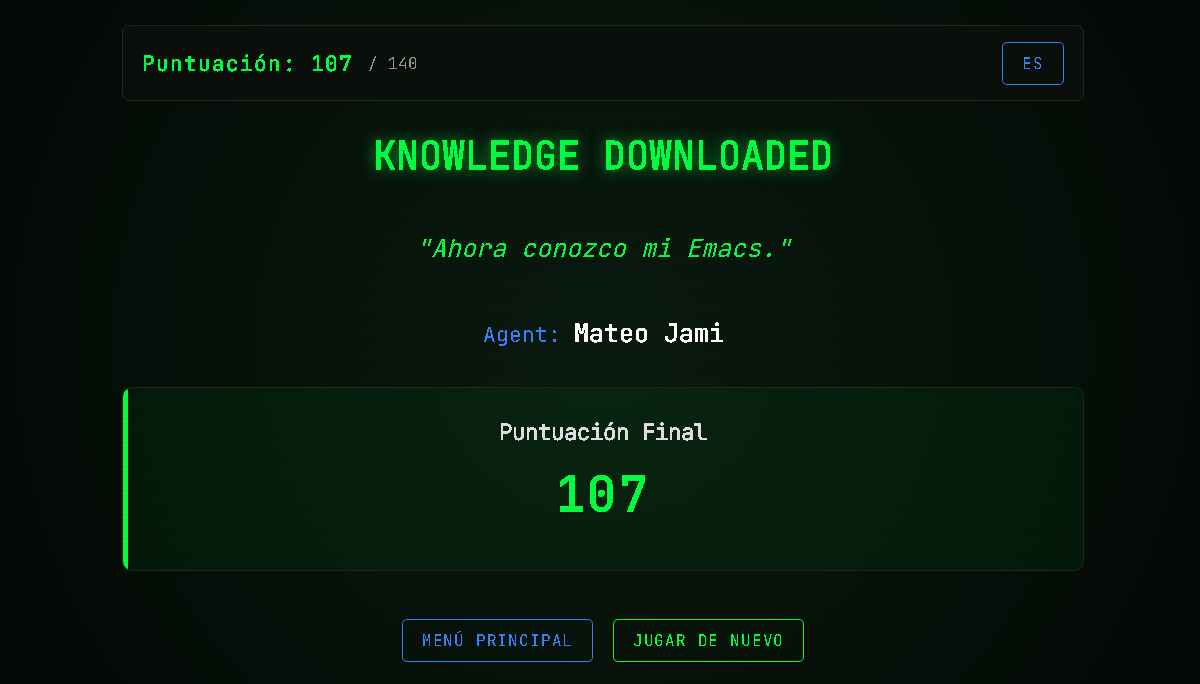
\includegraphics[width=.9\linewidth]{images/ImagenUnoMJ.png}
\end{center}
\begin{center}
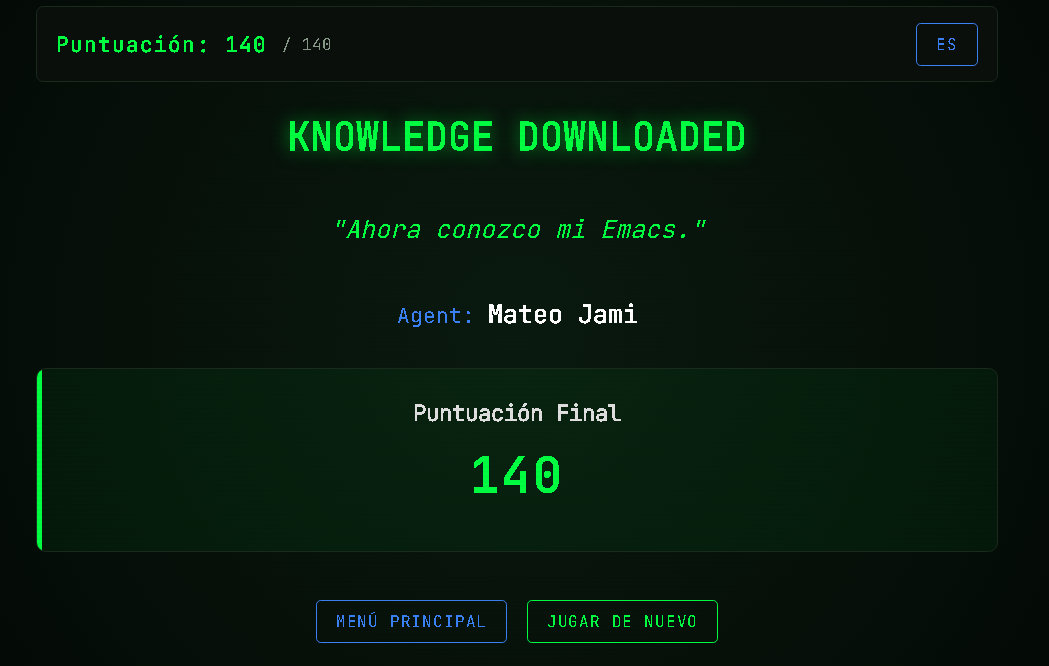
\includegraphics[width=.9\linewidth]{images/ImagenDosMJ.png}
\end{center}
\begin{center}
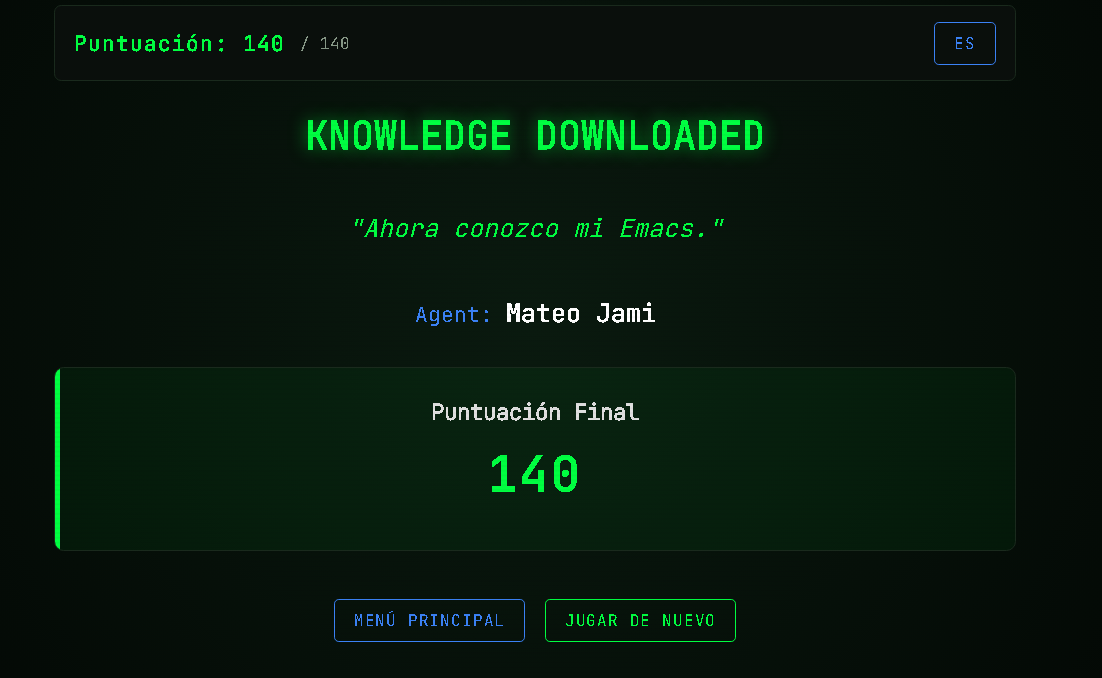
\includegraphics[width=.9\linewidth]{images/ImagenTresMJ.png}
\end{center}


Alex Flores: 
\begin{center}
\begin{tabular}{rr}
\hline
iteración & Puntaje\\[0pt]
\hline
1 & 100\\[0pt]
2 & 110\\[0pt]
3 & 140\\[0pt]
\hline
\end{tabular}
\end{center}

\begin{center}
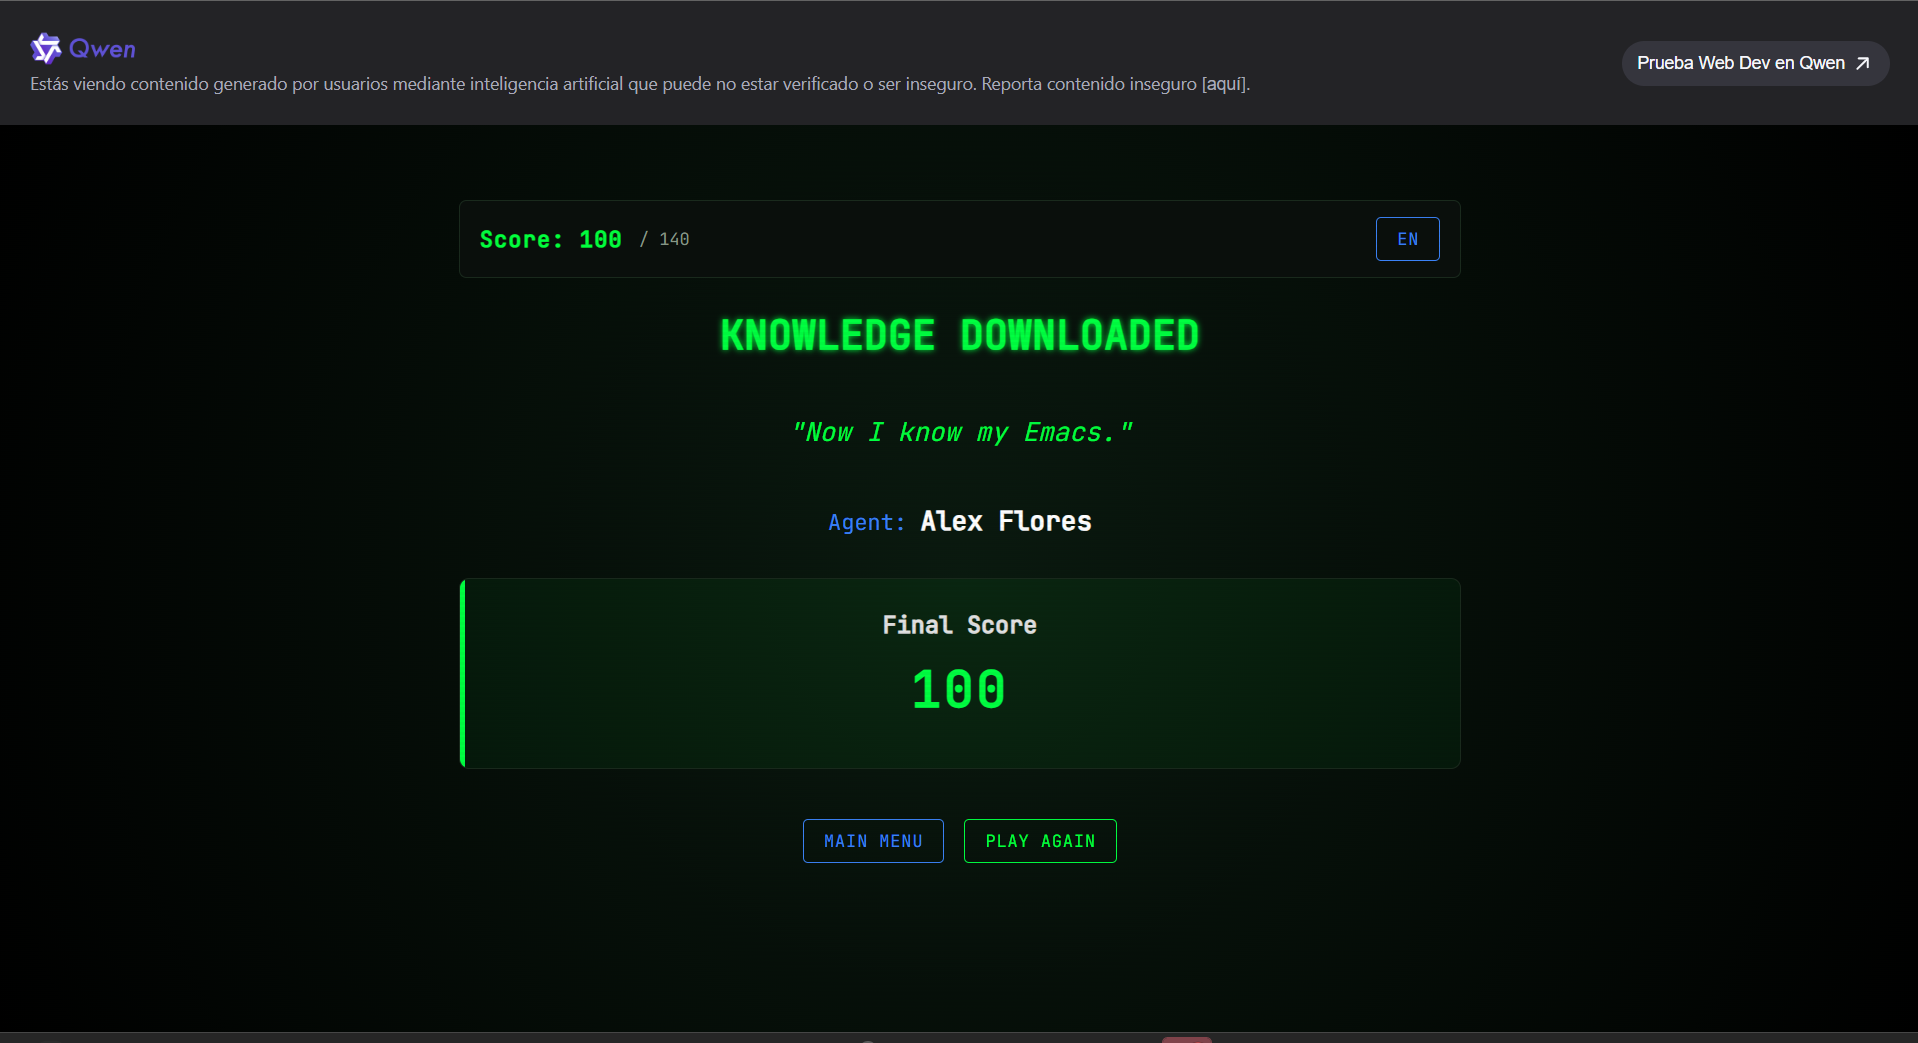
\includegraphics[width=.9\linewidth]{./images/Alex_game1.jpeg}
\end{center}
\begin{center}
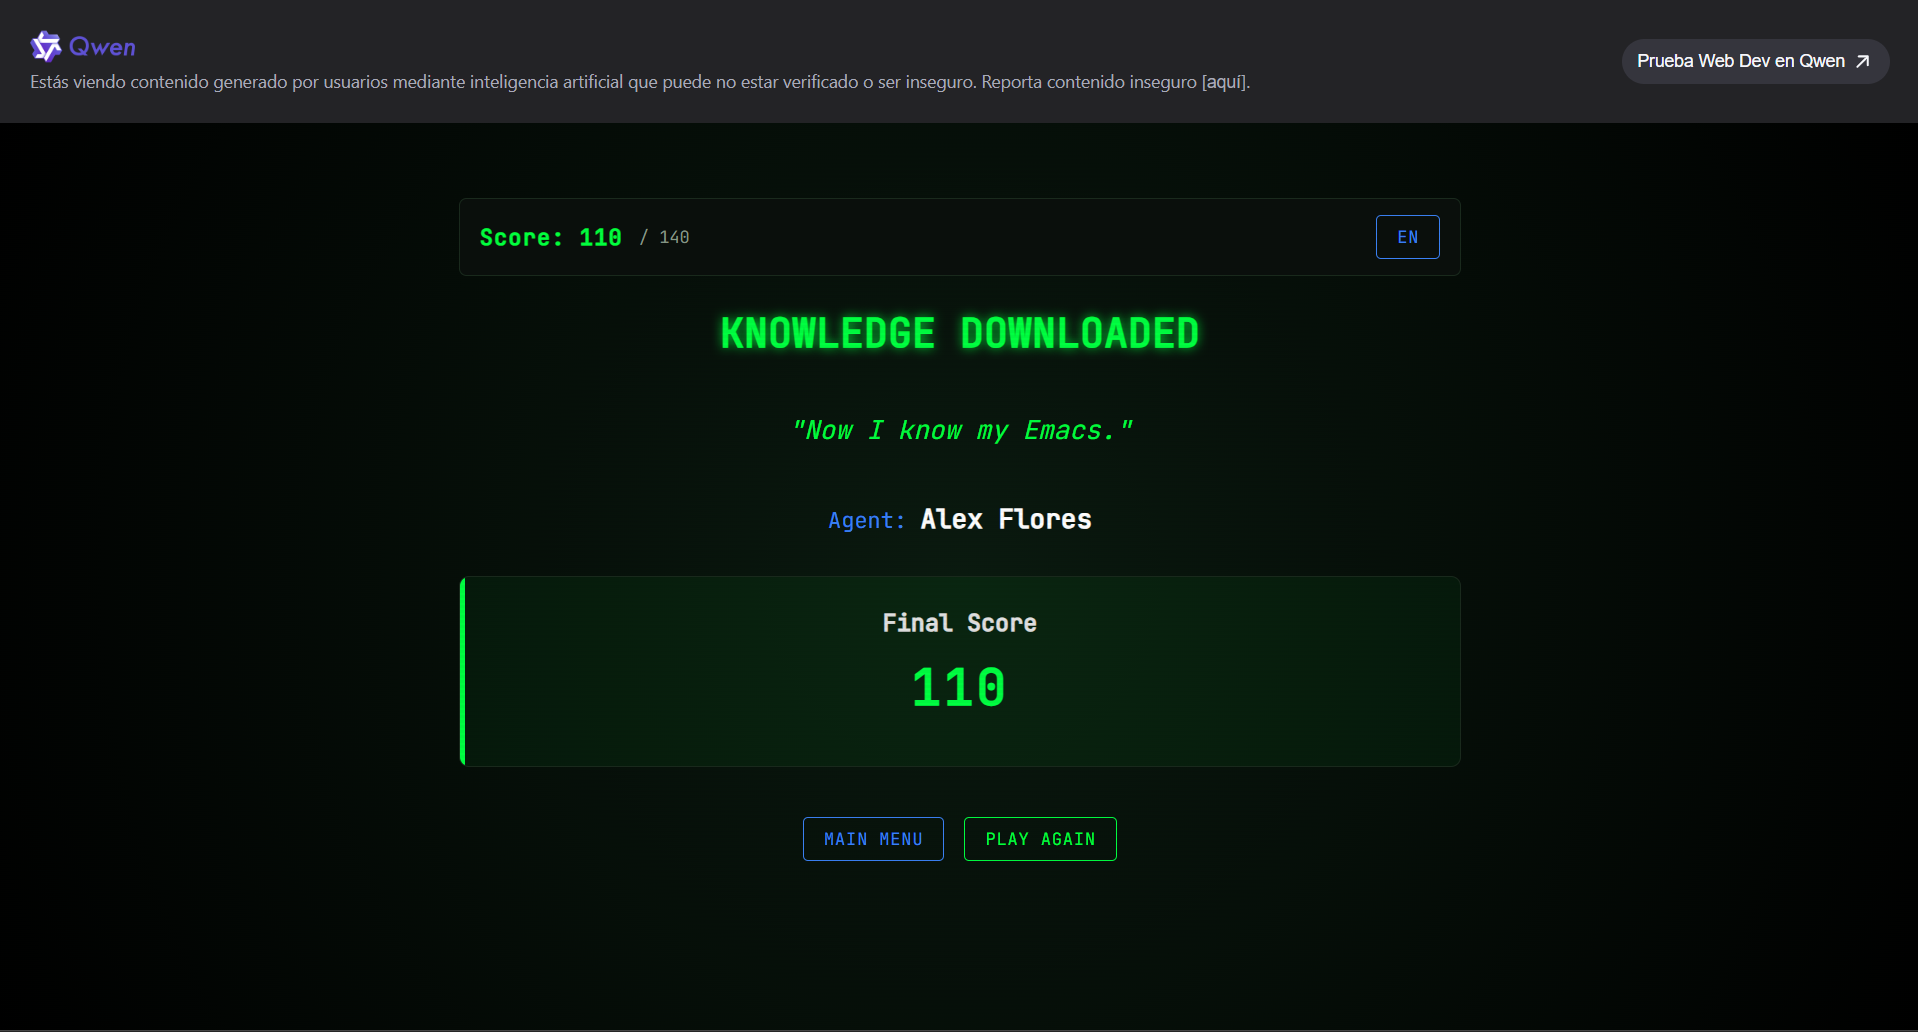
\includegraphics[width=.9\linewidth]{./images/Alex_game2.png}
\end{center}
\begin{center}
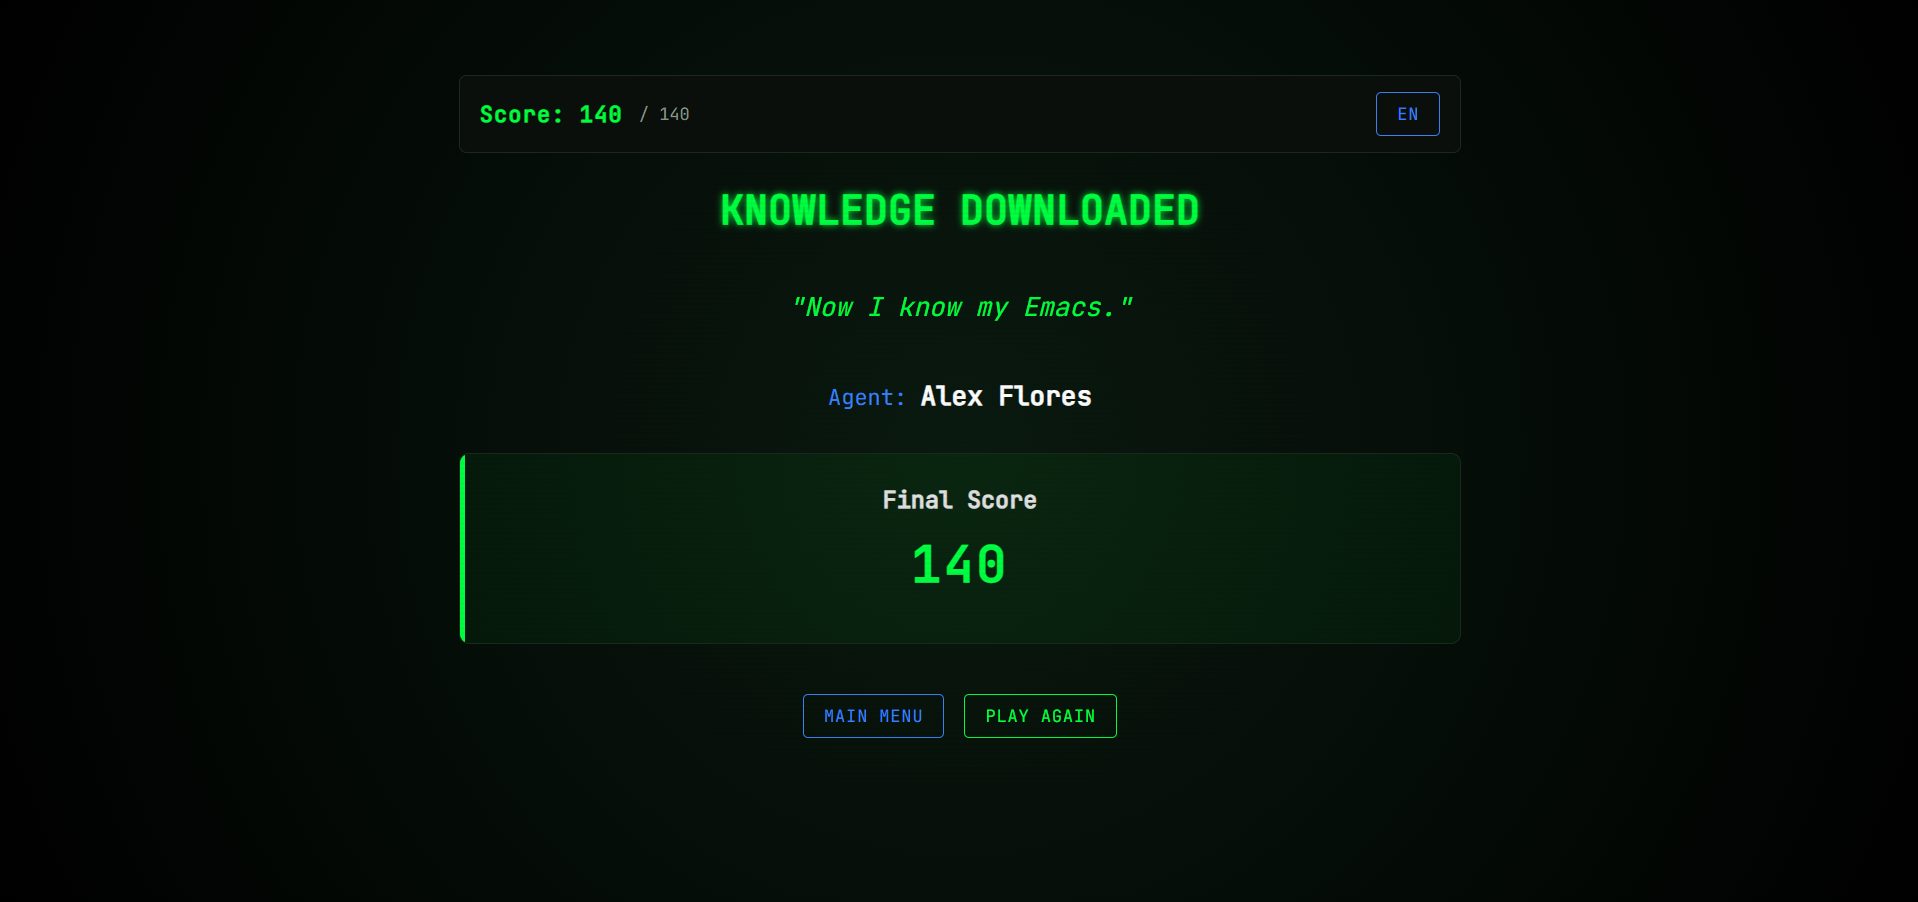
\includegraphics[width=.9\linewidth]{./images/Alex_game3.png}
\end{center}

Molina Jhanavi: 
\begin{center}
\begin{tabular}{rr}
\hline
iteración & Puntaje\\[0pt]
\hline
1 & 124\\[0pt]
2 & 140\\[0pt]
3 & 140\\[0pt]
\hline
\end{tabular}
\end{center}

\begin{center}

\includegraphics[width=.9\linewidth]{Puntaje1.png}
\end{center}
\begin{center}
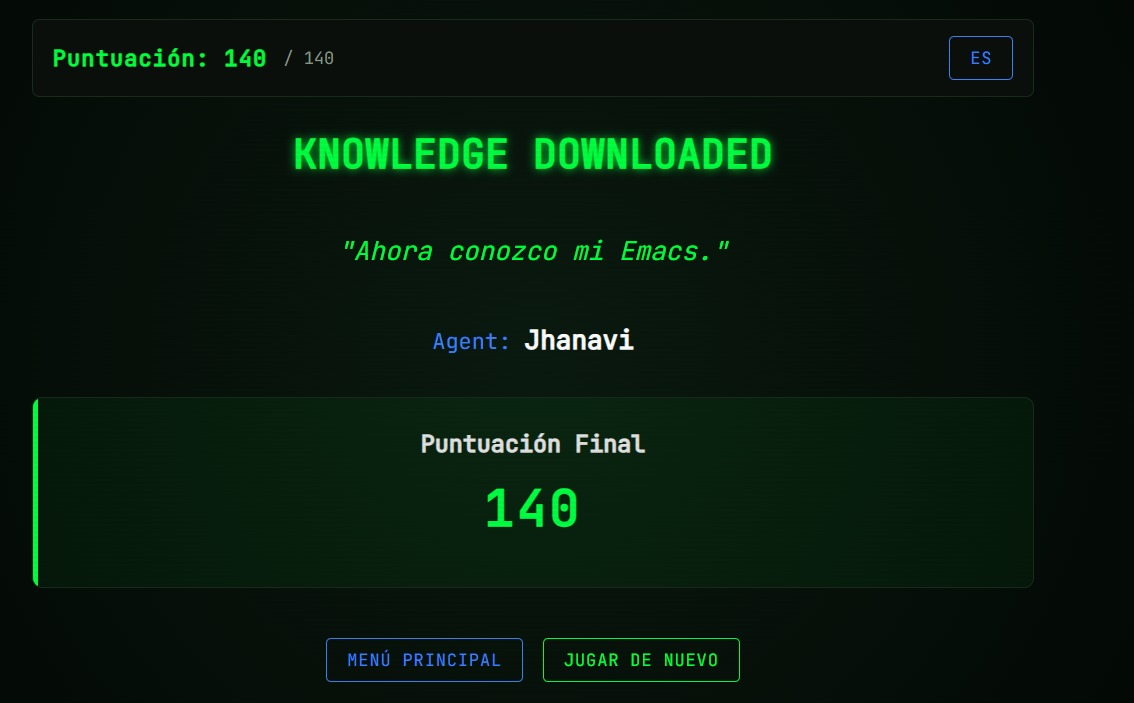
\includegraphics[width=.9\linewidth]{Puntaje2.png}
\end{center}
\begin{center}
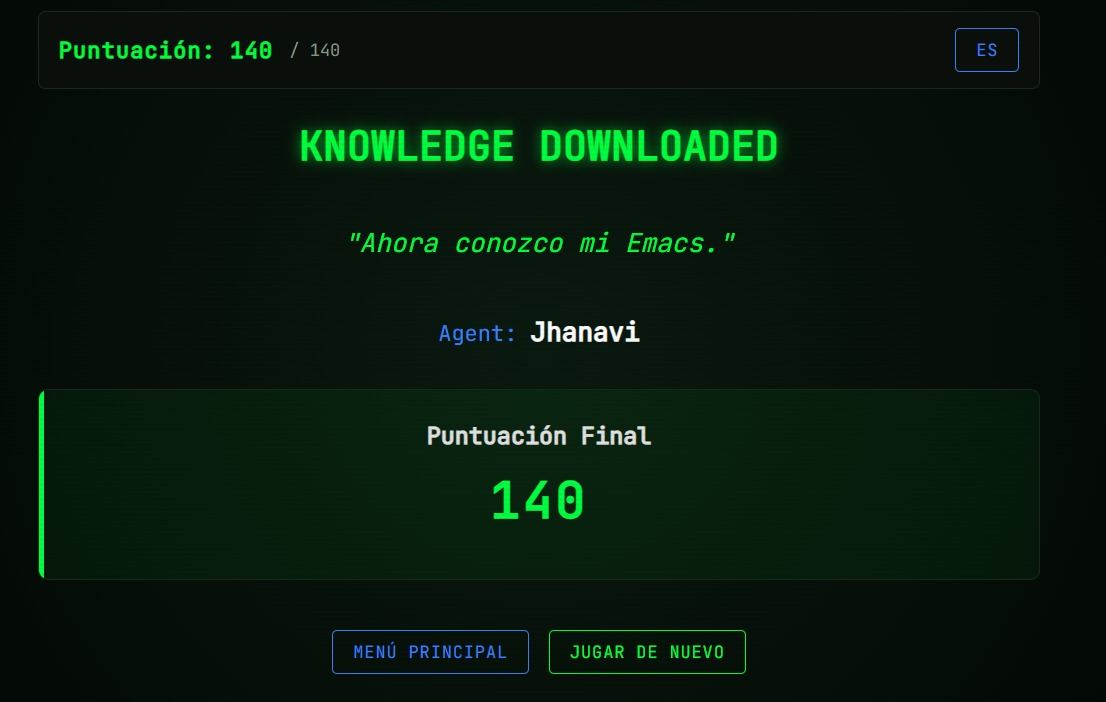
\includegraphics[width=.9\linewidth]{Puntaje3.png}
\end{center}

Sagñay Micaela: 
\begin{center}
\begin{tabular}{rr}
\hline
iteración & Puntaje\\[0pt]
\hline
1 & 128\\[0pt]
2 & 140\\[0pt]
3 & 140\\[0pt]
\hline
\end{tabular}
\end{center}

\begin{center}
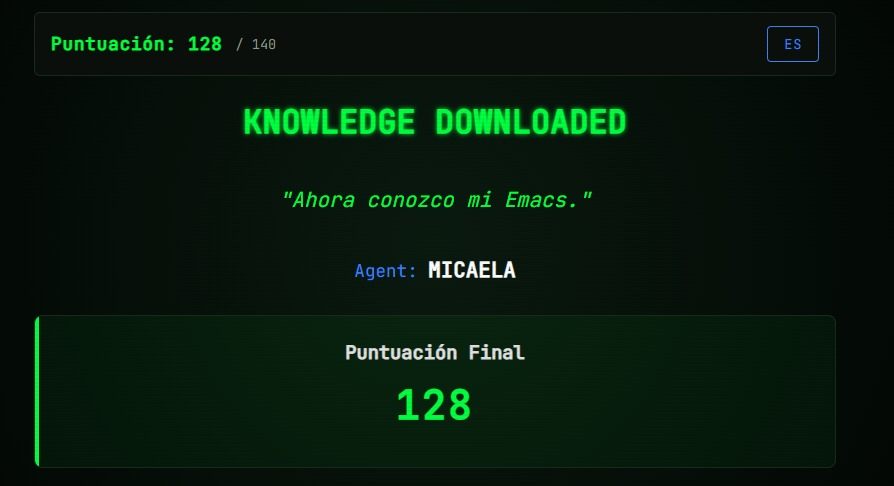
\includegraphics[width=.9\linewidth]{./Juego1.png}
\end{center}
\begin{center}
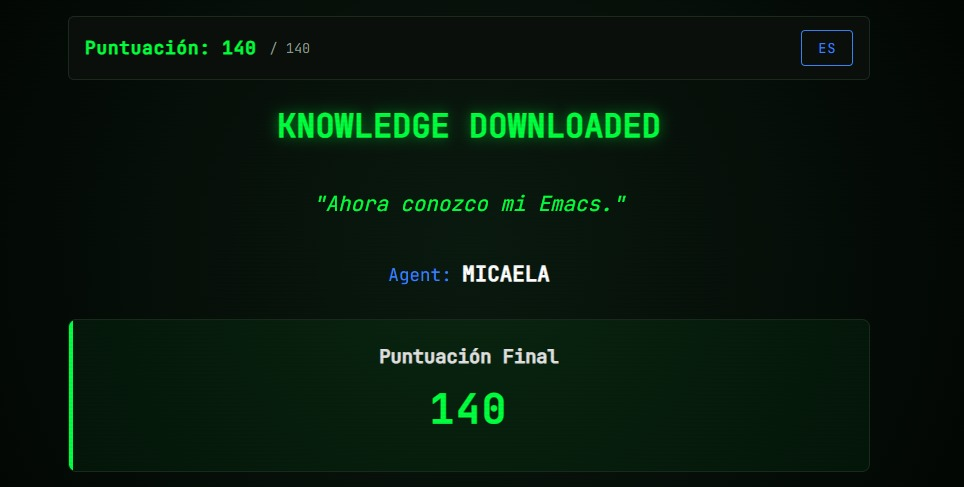
\includegraphics[width=.9\linewidth]{./Juego2.png}
\end{center}
\begin{center}
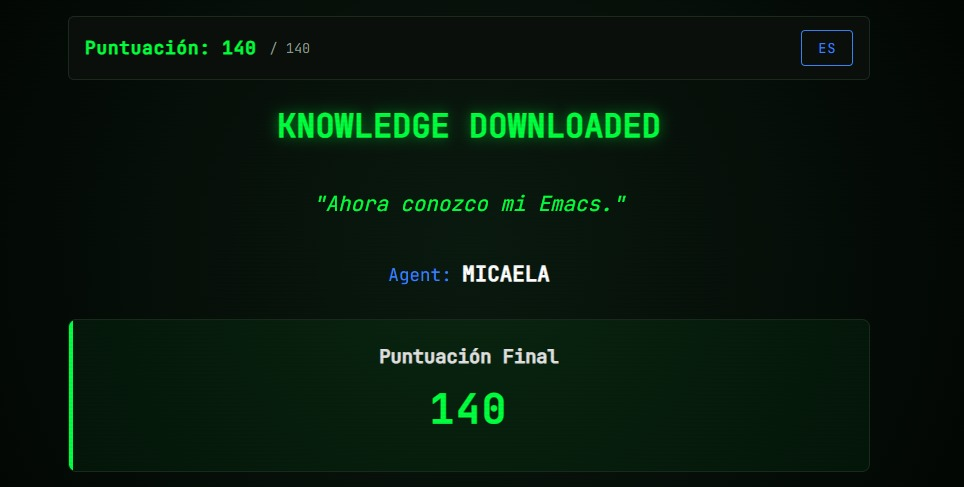
\includegraphics[width=.9\linewidth]{./Juego3.png}
\end{center}


\subsection{Usando Emacs para tener Ayuda sobre Emacs}
\label{sec:orgee5efbd}
¿Qué comandos le resultan más fáciles de usar y cuáles le son más
extraños? Identifique 4 comandos que le sean fáciles y 4 que le
resulten complicados. Revise qué dice la ayuda de Emacs sobre cada
comando y escriba en sus palabras el para qué sirve.

Para consultar lo que hace un comando ejecute:
\begin{enumerate}
\item \texttt{C-h k}
\item Emacs le preguntara cuál es la combinación de la que requiere
ayuda. Presione las teclas del comando. Por ejemplo, \texttt{C-x C-f}
\item Emacs abrirá un nuevo buffer con la descripción del comando.
\item Cambie al buffer de la ayuda con \texttt{C-x o}
\item Seleccione el primer parrafo de ayuda ubicando el cursor al inicio
del parrafo y activando la marcación de texto con
\texttt{C-SPC}. Seleccione avanzando por palabras \texttt{M-f} o directamente
toda la linea \texttt{C-e}
\item Una vez seleccionado, copie el texto con \texttt{M-w}.
\item Regrese al buffer anterior con \texttt{C-x o}.
\item Pegue el texto en <Pegar lo que dice el\ldots{}> con \texttt{C-y}
\end{enumerate}

\textbf{\textbf{Comandos Fáciles}}
\begin{enumerate}
\item \textbf{\textbf{Mateo Jami:}} <C-x-C-s>. <C-x C-s runs the command save-buffer (found in global-map), which is
\end{enumerate}
an interactive native-compiled Lisp function in ‘files.el’.>
\begin{enumerate}
\item \textbf{\textbf{Alex Flores:}} <C-x C-f>. <C-x C-f runs the command find-file (found in global-map), which is an interactive native-compiled Lisp function in ‘files.el’. It is used to open or create files in Emacs.>
\item \textbf{\textbf{Molina Jhanavi:}} \texttt{C-x C-f} Cambiar a un búfer visitando el archivo NOMBRE\textsubscript{ARCHIVO}, creando uno si no existe ninguno
\item \textbf{\textbf{Sagñay Micaela:}} Me resultó súper sencillo usar \texttt{C-x C-f} para abrir archivos, \texttt{C-s} para buscar, \texttt{C-x C-s} para guardar, \texttt{C-g} para cancelar y \texttt{M-w} para copiar.
\end{enumerate}

\textbf{\textbf{Comandos Difíciles}}
\begin{enumerate}
\item \textbf{\textbf{Mateo Jami:}} <C-x-b>. <C-x b runs the command switch-to-buffer (found in global-map), which
\end{enumerate}
is an interactive native-compiled Lisp function in ‘window.el’.>
\begin{enumerate}
\item \textbf{\textbf{Alex Flores:}} <C-h k>. <C-h k runs the command describe-key
(found in global-map), which is an interactive native-compiled Lisp
function in ‘help.el’. It displays documentation for the key sequence you press next, showing what command it is bound to and what it does.>
\item \textbf{\textbf{Molina Jhanavi:}} \texttt{C-s} El comando isearch-forward (que se encuentra en global-map), que es una función Lisp interactiva compilada de forma nativa en 'isearch.el'
\item \textbf{\textbf{Sagñay MIcaela:}} Se me complicó bastante usar \texttt{C-x o} para cambiar de ventana, \texttt{M-\%} para reemplazar, \texttt{C-x u} para deshacer y \texttt{M-x} para ejecutar funciones.
\end{enumerate}
\section{Equipo de Trabajo}
\label{sec:org591ca56}
Complete la información de los integrantes de grupo e indique el líder
de grupo. Por defecto será la primera persona designada en la lista compartida.

\begin{center}
\begin{tabular}{lll}
\hline
Nombre & email & Rol\\[0pt]
\hline
Jami Mateo & mateo.jami@epn.edu.ec & líder\\[0pt]
Sagñay Micaela & micaela.sagnay@epn.edu.ec & colaborador\\[0pt]
Molina Jhanavi & jhanavi.molina@epn.edu.ec & colaborador\\[0pt]
Flores Alex & alex.flores01@epn.edu.ec & colaborador\\[0pt]
\hline
\end{tabular}
\end{center}

\section{Verificación de Entregables [100\%]:}
\label{sec:orgf255697}
Ejecute \texttt{C-c C-c} sobre los ítems de tarea según se hayan cumplido o
no. Si un ítem no pudo realizarse apunte en la siguiente sección las
razones al respecto.
\begin{itemize}
\item[{$\boxtimes$}] Verificación de configuración de entorno WSL y paquetes del curso.
\item[{$\boxtimes$}] Tutorial de Comandos Emacs realizado.
\item[{$\boxtimes$}] Captura de Imágenes y puntajes de Emacs Trainer App.
\item[{$\boxtimes$}] Usando Emacs para tener ayuda sobre Emacs
\item[{$\boxtimes$}] Verifique que estén los nombres de los integrantes del equipo e
identificado el líder.
\item[{$\boxtimes$}] Revisión de ortografía con \texttt{ispell} en el buffer
\item[{$\boxtimes$}] Generación de Archivo PDF \texttt{M-x org-latex-export-to-pdf}
\item[{$\boxtimes$}] Subir al aula virutal archivo \texttt{.org} y \texttt{.pdf}
\end{itemize}
\subsection{Problemas con la Tarea/logísticos:}
\label{sec:orgd5bad0e}
\begin{itemize}
\item Sin novedad de problemas con las tareas.
\end{itemize}
\end{document}
